\caption{This table is showing the required bandwidth for each application (KiloBytes per core per second). $ReqBW_x = TraceSize_x (KB) / (\# of cores)_x / Runtime_x (S)$
Because of the crashing problems of Callgrind on \textit{C} input and 64 nodes, I only include \textit{B} input and 1, 4, and 16 nodes results. Clearly ParLOT(main) is beating Callgrind while they both generate the same information (I still believe ParLOT(main) generated traces are more informative and rich). ParLOT(all) bandwidth is the highest but with capturing all of the function calls within a single execution, there is no surprise. Another interesting fact from this table is, for ParLOT(main), bandwidth drops from \textbf{0.62} for 16 cores to \textbf{0.27} for 256 cores (good scalability). It is the opposite for Callgrind where the required bandwidth jumps from \textbf{3.28} (KB/s) for 16 cores to \textbf{33.06} (KB/S) for 256 cores. I also have the results of required bandwidth of ParLOT for 64 nodes(1024 cores) and Input C but I did not include them here because I did not have them for Callgrind (explained above).  Fig \ref{chartAvg_bw_B_p3_5} visualize these numbers (Average values)}


\begin{figure*}[!t]
\centering
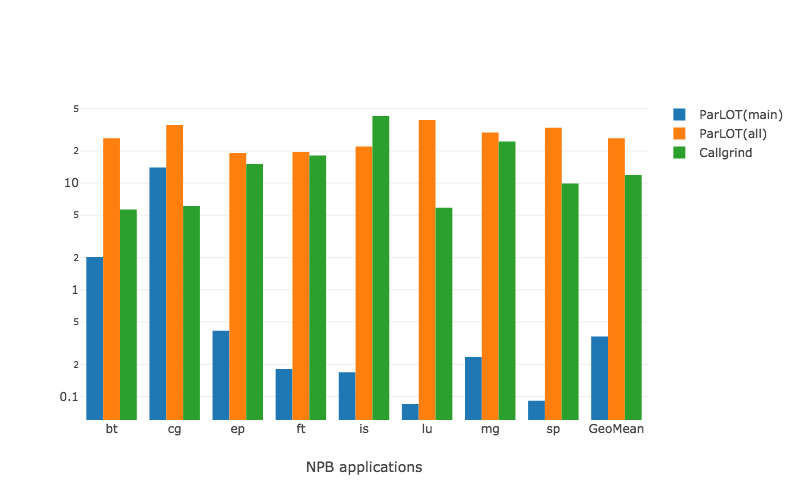
\includegraphics[width=5in]{figs.psc/chartAvg_bw_B_p3_5.png}
\caption{ Required Bandwidth (KB) per core per second for ParLOT and Callgrind.  
(Input: B)}
\label{chartAvg_bw_B_p3_5}
\end{figure*}